\appendix
\UnnumberedChapter{PHỤ LỤC}

\section*{Phụ lục 1. Ảnh mẫu của 43 lớp}

Mỗi hàng là một lớp: cột đầu là ảnh biển chuẩn (thư mục \texttt{Meta}), năm cột sau là ảnh ngẫu nhiên từ tập Train.

\begin{figure}[H]
    \centering
    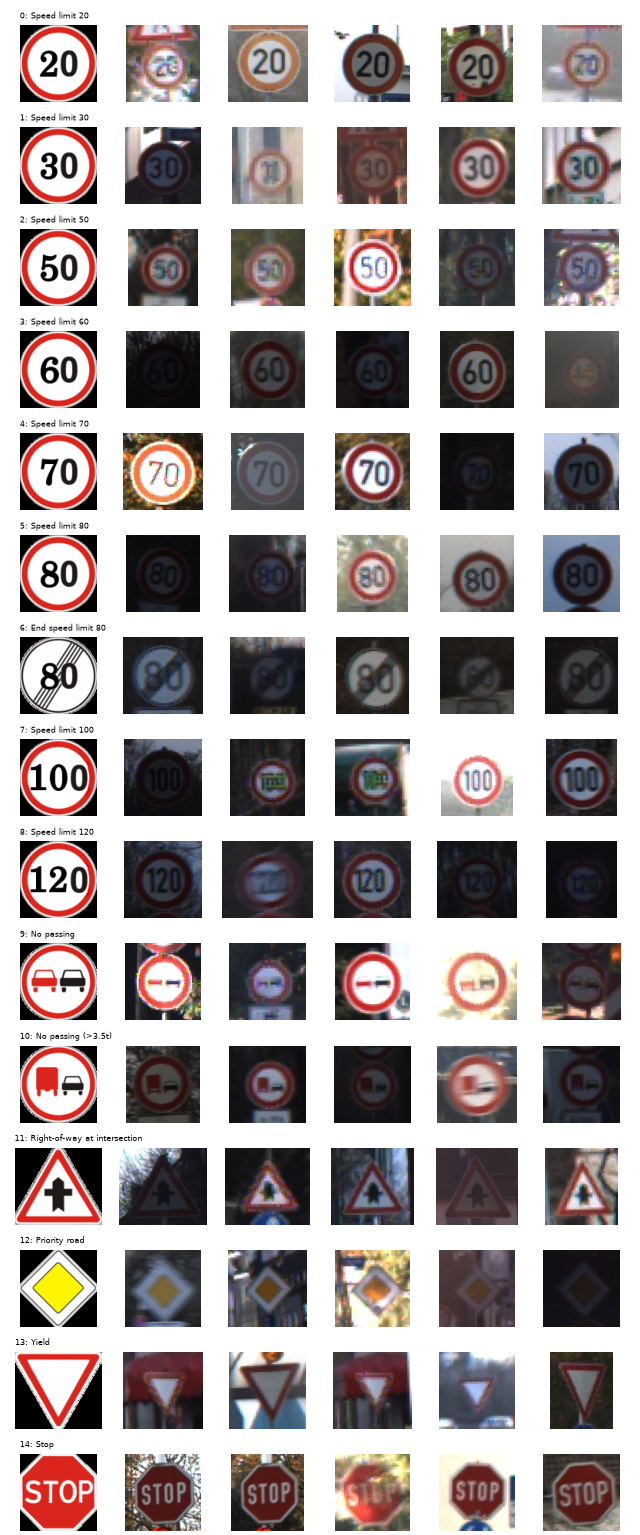
\includegraphics[width=0.325\textwidth]{images/eda_samples_1.png}\hfill
    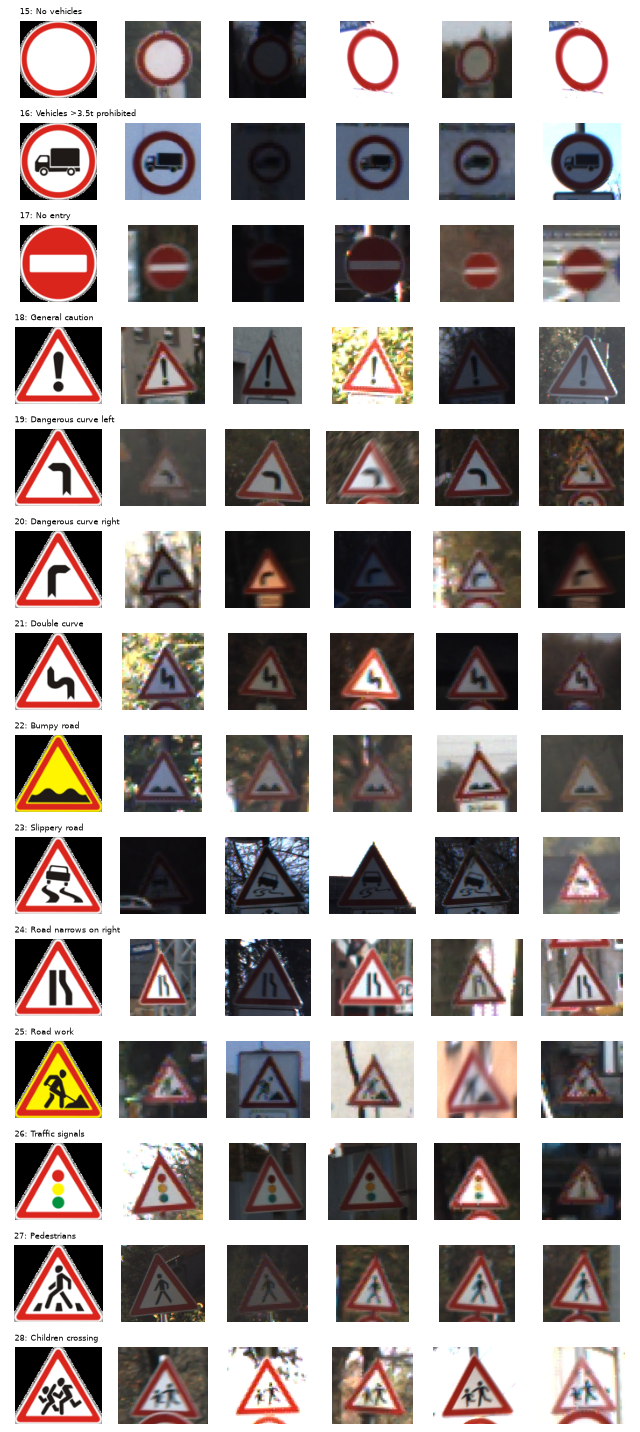
\includegraphics[width=0.325\textwidth]{images/eda_samples_2.png}\hfill
    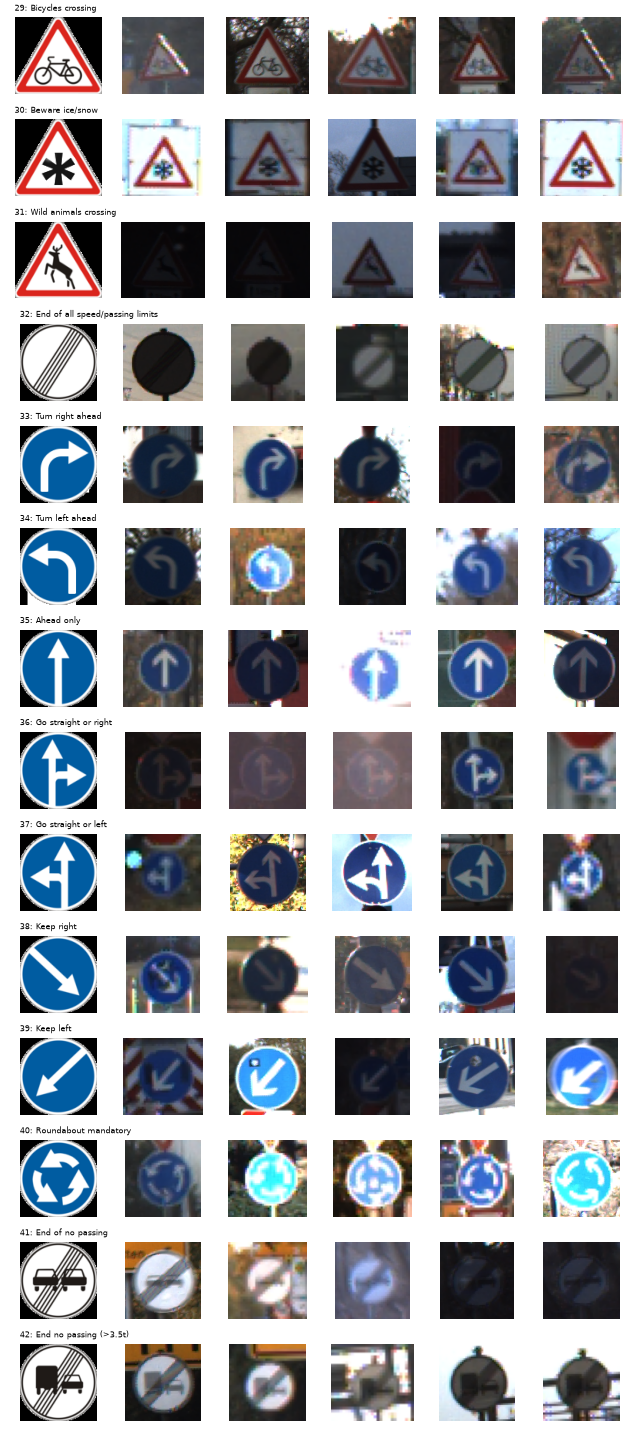
\includegraphics[width=0.325\textwidth]{images/eda_samples_3.png}
    \caption*{Hình PL1. Ảnh mẫu của 43 lớp biển báo (lớp 0 đến 14, 15 đến 28, 29 đến 42)}
    \Nguon{Nhóm vẽ từ bộ dữ liệu GTSRB}
\end{figure}

\section*{Phụ lục 2. Khai báo sử dụng công cụ AI}

Em có sử dụng công cụ AI (Claude, Anthropic) để hỗ trợ trong quá trình thực hiện bài tập lớn, cụ thể: rà soát mã nguồn và kết quả, hướng dẫn cài đặt và chạy chương trình, soạn bản nháp tệp README, tệp khai báo thư viện và khung báo cáo LaTeX theo template của học phần, gợi ý các giả thuyết giải thích kết quả. Em đã tự chạy lại toàn bộ quy trình hai lần và đối chiếu kết quả, đọc lại mã nguồn, số liệu và nội dung báo cáo, và chỉnh sửa trước khi nộp. Chi tiết ghi ở tệp \texttt{AI\_USAGE.md} trong repository.

\section*{Phụ lục 3. Phân công công việc}

\begin{table}[H]
\centering
\caption*{Bảng PL1. Phân công công việc của nhóm}
\begin{tabular}{|p{4.4cm}|p{3cm}|p{7.6cm}|}
\hline
\textbf{Thành viên} & \textbf{MSV} & \textbf{Công việc} \\
\hline
Dương Duy Khánh & 1871020326 & {Toàn bộ} \\
\hline
\end{tabular}
\end{table}

\section*{Phụ lục 4. Mã nguồn và liên kết liên quan}

\begin{itemize}
    \item Repository GitHub của nhóm: \url{https://github.com/KhanhD613/learn-git}.
    \item Các tệp kết quả: thư mục \texttt{results/} trong repository (bảng CSV, hình, nhật ký chạy).
    \item Hướng dẫn cài đặt và chạy lại: tệp \texttt{README.md} trong repository.
\end{itemize}
